\documentclass{article}
\usepackage[utf8]{inputenc}
\usepackage{graphicx}
\usepackage[pages=some]{background}
\usepackage[nottoc]{tocbibind}
\usepackage{fancyhdr}
\usepackage{cmap}
\usepackage[english,ngerman]{babel}
\usepackage{iflang}

\setlength{\parindent} {0pt} %Entfernung der automatischen Einrückung

%\usepackage{showframe}
% +------------------------------------------------------------------------------+ %
% | ADD PACKAGES HERE IF YOU NEED THEM                                           | %
% +------------------------------------------------------------------------------+ %
\usepackage{todonotes}
\usepackage{textcomp}
\usepackage{amsmath}
\usepackage[left=2.5cm,right=2.5cm]{geometry}
\usepackage{amssymb}
\usepackage{physics}
\usepackage{graphicx}
\usepackage{color}
\usepackage{sidecap}
\usepackage{floatrow}
\usepackage{algorithm}
\usepackage[noend]{algpseudocode}
% +------------------------------------------------------------------------------+ %
% | DO NOT CHANGE THE REST OF THIS DOCUMENT                                      | %
% +------------------------------------------------------------------------------+ %

\backgroundsetup{
firstpage=true,
placement=bottom,
scale=1,
color=black,
opacity=0.4,
angle=0,
contents={%
  \makebox[\paperwidth]{\hspace*{\fill}
\includegraphics[width=.6\paperwidth]{images/lmu_seal}}%
  }%
}

\widowpenalty10000
\clubpenalty10000

\begin{document}
% +------------------------------------------------------------------------------+ %
% | EDIT THESE SETTINGS ACCORDING TO YOUR THESIS                                 | %
% +------------------------------------------------------------------------------+ %

\newcommand{\seminar}{Trends in Mobilen und Verteilten Systemen}

\newcommand{\authorA}{Nadja Heinecke}
\newcommand{\authorB}{Christopher Sorg}
\newcommand{\authorC}{Daniel Seidl}
\newcommand{\supervisor}{Leo Alexander Sünkel}

\newcommand{\thesistitle}{Quantum Machine Learning - Ideal und Wirklichkeit}

\newcommand{\thesisabstract}{% \/ put your thesis abstract below \/
Diese Arbeit soll die Möglichkeiten der Nutzung von Quanten Computern für Machine Learning Algorithmen erforschen. Hierfür wollen wir zunächst ein paar Grundlagen des Quantum Computing für den Leser auffrischen, bevor wir auf Nutzungsbeispiele eingehen. Insbesondere soll aber auch die Anwendbarkeit auf in den nächsten Jahren realisierbaren, sogenannten Noisy Intermediate-Scale Quantum (NISQ) Computern beleuchtet werden. 
\\Wir möchten hiermit einen Überblick über lang- und kurzfristige Ziele des Quantum Machine Learnings und deren Umsetzbarkeit bieten.
}

\newcommand{\thesisauthorship}{% \/ describe who wrote what below \/
\authorB $\,$ hat die Kapitel \ref{sec:qgmc} und \ref{sec:disc} verfasst.\\
\authorC \ hat Kapitel \ref{sec:conclusion} und gemeinsam mit \authorA \ die Kapitel \ref{sec:intro} und \ref{sec:nisq} verfasst.
}


\selectlanguage{ngerman} 

\let\oldcontentsname\contentsname
\renewcommand{\contentsname}{\centering\small\oldcontentsname}

\title{\thesistitle}
\author{\authorA \IfLanguageName{ngerman}{und}{and} \authorB}
\date{\today}

\begin{titlepage}
	\centering
    \BgThispage
    \vspace*{-\topmargin}\vspace{-1in}%
    \vspace*{-\headheight}\vspace{-\headsep}%
    \vspace*{-\topskip}%
    \hspace*{-\oddsidemargin}
    \hspace*{-\marginparsep}
    \hspace*{-\marginparwidth}
    %\hspace{\textwidth}%
	\makebox[\paperwidth]{\centering
\includegraphics[width=.95\paperwidth]{images/lmu_header}}
	\vspace*{1.75cm}
	\par
	{\scshape\large \seminar\par}
	{\huge\bfseries\thesistitle\par}
	\vspace*{1.75cm}
	\large \begin{tabular}{ l l }
	  \textsc{Bearbeiter}:&{\authorA}\\
	  &{\authorB}\\&{\authorC}\\
	  \\
	  \textsc{Betreuer:}&{\supervisor}\\
	  \\
	  \textsc{Aufgabensteller:}&{Prof. Dr. Claudia Linnhoff-Popien}\\
	\end{tabular}
	\par
	\vspace*{1.75cm}
	\begin{otherlanguage}{ngerman}
		{\large Dokument erstellt\par\today\par}
	\end{otherlanguage}
	\newpage
	\thispagestyle{empty}
	\mbox{}
	\newpage
\end{titlepage}
\cleardoublepage

\begin{center}
	\LARGE
	\thesistitle
\end{center} 
\vspace*{.75cm}
\begin{abstract}
\noindent\thesisabstract
\end{abstract}
\vspace*{.75cm}
\tableofcontents
\newpage
\thispagestyle{empty}
\mbox{}
\newpage
\cleardoublepage


%Anmerkung, da Fehler beim Kompilieren: Zeichen wie \ oder & sind in LaTeX Commandchars, müssen also bei normaler Benutzung mit \( \) oder $$ escapet werden - Chris

%TO DO 
%Anwendungsfälle zitieren hier evtl aus 1611 Matrix + Fourier transformationen
%mehr zu unlösbaren/langen Berechnungen
%mehr Quantum Machine Learning
\section{Einleitung}
\label{sec:intro}
Machine Learning (ML) scheint im Zeitalter der Informationstechnologie eine der großen und vielversprechenden „Killer“ Applikationen zu sein. Schon heute reichen die Anwendungsgebiete von Verkehr $\&$ Mobilität, über Marketing, Recht und Verwaltung bis hin zum Gesundheitswesen \cite{opportunitieschallenges1}. ML wird für Bilderkennung, Stimmungsanalyse, Videoüberwachung und auch für die tägliche E-Mail Klassifizierung und Spam-Filterung verwendet. Entsprechende Algorithmen ermöglichen dabei durch Mustereingaben das Erlernen verschiedener Anwendungsfälle, anstatt einer vordefinierten Vorgangsanweisung \cite{quantummethodssupervised1}. \\

\\
Viele Aufgabengebiete sind auch mit heutigem Technologiestandard – mit immer steigender Rechenleistung der Computersysteme – nur mit sehr großem Zeit-, Rechen- und somit auch Energieaufwand lösbar, manche dieser Probleme sind sogar so komplex, dass die Berechnung hierfür entweder Jahre dauern würde, oder diese sogar komplett unlösbar sind \cite{fraunhoferbigdata}.\\
Quanten Computing bietet eine ganz andere Herangehensweise an die Berechnung solcher sehr kostenintensiven Probleme. Durch die echte Parallelität, die Quanten Computer bei der Berechnung versprechen, dürfte es möglich sein, mehrere Lösungsansätze und -wege gleichzeitig zu berechnen und somit wesentlich größere Datenbestände in einem kürzeren Zeitfenster abzuarbeiten.\\
Es ist zu erwarten, dass Quanten Computing sofern es diese Versprechungen tatsächlich erfüllt, eine Revolution in der Informationstechnik einleiten wird. Die Frage bleibt bloß, in welchen Bereichen sich diese neue Technik besonders gut einsetzen lässt und für welche sich klassische Computer weiterhin besser eignen. \\
\\
Im Rahmen dieser Arbeit soll nun die  Einbindung von Quanten Computern im Bereich des Machine Learnings genauer betrachtet werden, insbesondere die kurzfristige Umsetzung des Quantum Machine Learnings (QML) in den kommenden Jahren.\\
Da ML-Algorithmen allgemein zu den komplexeren und kostenintensiven Berechnungen gehören, könnte es sich hierbei um einen idealen Anwendungsbereich für Quanten Computer handeln. Wie kann dies also umgesetzt werden, und wird es in der nahen Zukunft bereits möglich sein solche Quanten Machine Learning Algorithmen zu realisieren?\\
In diesem Sinne sollen hier zunächst die Grundlagen des Quantum Gate Models, sowie die Chancen die sich daraus potentiell in Zukunft für ML-Algorithmen ergeben, betrachtet werden. \\
Da wir uns aber noch in der Anfangsphase der Entwicklung nutzbarer Quanten Computer befinden, soll im Folgenden auf die aktuelle Realität, zu überwindende Hürden und mögliche Lösungen dafür eingegangen werden. Insbesondere sollen hierbei Hybride Methoden, die auf einer Kombination aus klassischen und Quanten Computern aufbauen, betrachtet werden.\\
Insgesamt Soll diese Arbeit im Folgenden also einen Überblick schaffen über die möglichen, die bisherigen und zuletzt die in naher Zukunft erreichbaren technischen Fortschritte, die Quanten Computing für Machine Learning Algorithmen bietet.




\section{Quantum Gate Model}
\label{sec:qgmc}
In diesem Kapitel werden wir die im Titel der Arbeit angesprochene Idealumsetzung näher betrachten. In der derzeitigen NISQ-Ära (Stand 22.06.2021) entspricht dies leider noch überhaupt nicht der Wirklichkeit, hierzu folgt im Kapitel 3 dann mehr.
\subsection{Theoretische Grundlagen}
Bevor wir uns der tatsächlichen Umsetzung des Quantum Gate Models (QGM) widmen, sollten wir uns zunächst einmal der benötigten Grundlagen hierfür vertraut machen.\\
Grundlage des QGM ist die Quantenmechanik. Diese nanophysikalische Theorie entsprang der sogenannten Kopenhagener Interpretation von N. Bohr und W. Heisenberg 1927\cite[Seiten 108-111]{KopoBaker}.
Das zentrale Objekt hierbei ist eine sogenannte Wellenfunktion \(\Psi\)(\(\mathbf{r}\),t)\(\in \mathcal{H}(\mathbb{C}^n)\) zur Beschreibung aller Informationen eines Systems und als Lösung der Schrödingergleichung (Postulat von E. Schrödinger 1926), die wie folgt lautet\cite[Seite 22]{GriffithsQuantumMechanics}:
\begin{equation}
i \hbar \frac{\partial}{\partial t}\Psi(\mathbf{r},t) = \hat H \Psi(\mathbf{r},t)
\end{equation}
Hierbei seien \(i\) die imaginäre Einheit, \(\hbar\) das plank'sche Wirkungsquantum, \(\mathbf{r}\) der (mehrdimensionale) Ort und \( \hat H\) der selbst-adjungierte Hamiltonoperator (oder auch Energieoperator).\\
Nun lässt sich die Wellenfunktion mithilfe ihrer Eigenzustände darstellen. Diese werden meistens mit \(\Psi_n\) bezeichnet. Daraus resultiert die für die Quantenmechanik berühmte Dirac-Notation (nach P. Dirac)\cite[Seite 154]{GriffithsQuantumMechanics}:
\begin{align}
\ket{\Psi} &=: \begin{bmatrix}
           \Psi_{1} \\
           \Psi_{2} \\
           \vdots \\
           \Psi_{n}
         \end{bmatrix}
\text{("Ket"), } 
\bra{\Psi} =: (\Psi_{1}^* \,\Psi_{2}^*\, \cdot\cdot\cdot \Psi_{n}^*) \text{ ("Bra")}
\end{align}
Der Umstieg von klassischer auf quantenmechanische Physik wirkt sich natürlich auch auf das zugrundeliegende System aus. So werden nicht mehr wie bei klassischen Binärrechnern Bits verwendet, die entweder den Zustand 0 oder 1 annehmen können.
Vielmehr werden nun sogenannte Quantenbits - oder kurz Qubits - eingesetzt. Ein Qubit kann mehr als nur die Zustände 0 und 1 annehmen. Es kann auch die überlagerten Zustände annehmen, genauer\cite[Seite 20]{QuantumComputingHomeister}:
\begin{equation}
\text{Seien }\alpha, \beta \in \mathbb{C}.\text{ Dann gilt: }\ket{\Psi} = \alpha \cdot \ket{0} + \beta \cdot \ket{1} \text{ mit }|\alpha|^2 + |\beta|^2 = 1.
\end{equation}
Die Überlagerung dieser Zustände wird auch Superpostion genannt.\\
Erfolgt nun eine Messung des Qubits, so kollabiert die Wellenfunktion und das Qubit befindet sich mit Wahrscheinlichkeit \(|\alpha|^2\) im Zustand \(\ket{0}\) und \(|\beta|^2\) im Zustand \(\ket{1}\)\cite[Seite 20]{QuantumComputingHomeister}.\\

Wie im klassischen Sinne, werden Qubits natürlich auch in Gattern verbaut. Diese Gatter nennt man Quantum Gates. Grundlage dieser Gatter sind Matrizen M \(\in\) U(n) (Unitary Group).\\
\newpage
Wichtige Beispiele mit zugehörigem Gatter:\\
\begin{figure}[!htb]
\floatbox[{\capbeside\thisfloatsetup{capbesideposition={right},capbesidewidth=4cm}}]{figure}[\FBwidth]
{\caption{Die wichtigsten Gatter in einer Übersicht \cite{Gates}}\label{fig:test}}
{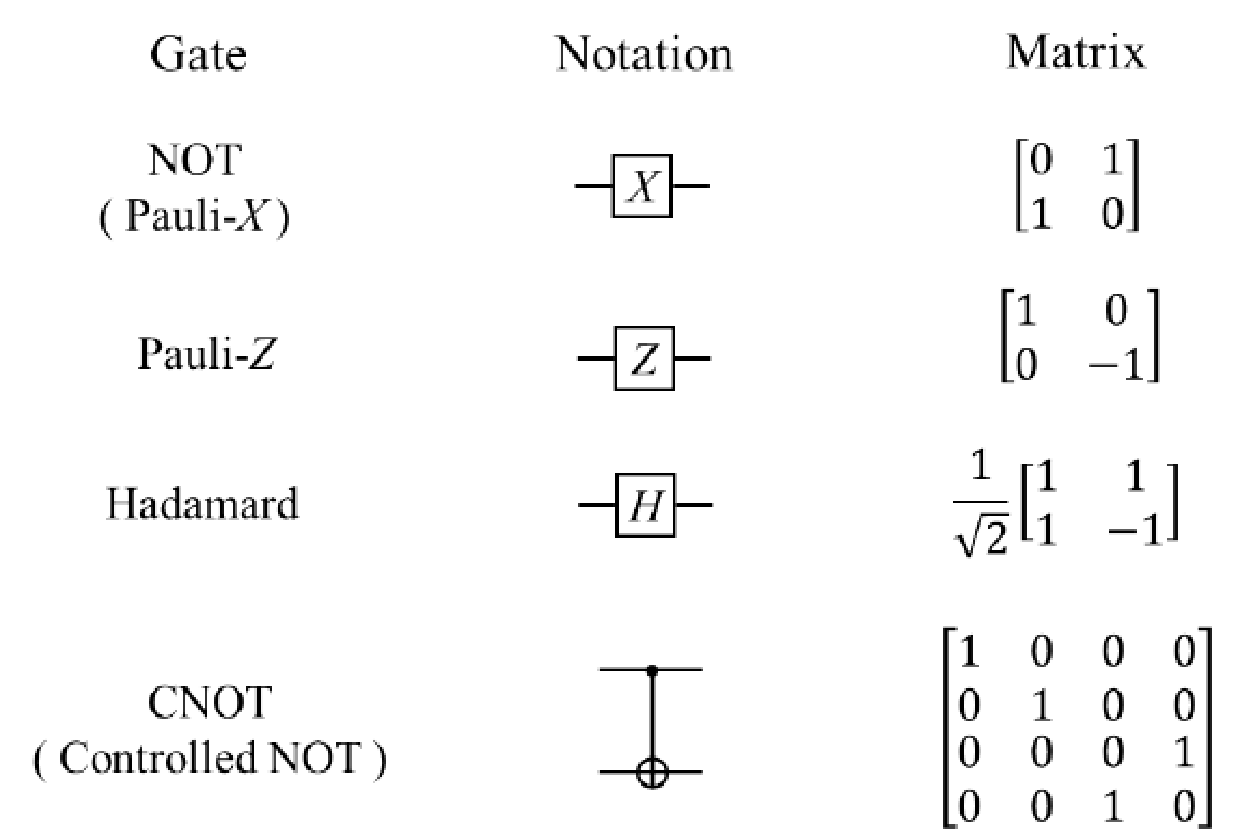
\includegraphics[width=11cm]{QML/images/gates.pdf}}
\end{figure}\\

Setzen wir nun mehrere Quantum Gates zusammen, erhalten wir - ähnlich wie im klassischen Sinne - sogenannte Quantenregister. Mathematisch kann man eine merkwürdige Eigenschaft dieser Quantenregister sehr schnell herleiten: Die sogenannte Verschränkung. Zunächst sei diese folgendermaßen definiert\cite[Seiten 53,55]{QuantumComputingHomeister}:\\

Sei $\ket{\Psi}$ der Zustand eines Quantenregisters mit n Bits (also folglich n Eigenzuständen), \(n \in \mathbb{N}\). Dieser Zustand heißt genau dann unverschränkt, wenn gilt:\\
\begin{equation}
    \ket{\Psi} = \ket{\Psi_{n-1}} \otimes \ket{\Psi_{n-2}} \otimes ... \otimes \ket{\Psi_{0}}
\end{equation}
Hierbei sei $\otimes$ logischerweise das Tensorprodukt zwischen den Eigenzuständen.\\
Der Zustand heißt folglich genau dann verschränkt, wenn keine solche Partitionierung existiert.\\
Merkwürdig erscheint hierbei nun intuitiv gesehen, dass eine Änderung eines Bits die Messung eines anderen Bits beinflusst, da die Eigenzustände miteinander verschränkt sind.\\

Zuletzt betrachten wir noch die wohl berümteste und gleichzeitig zentrale Folgerung aus der Quantenmechanik: Die Heisenbergsche Unschärferelation. Diese lautet wie folgt\cite{HeisenbergPascuzzo}:\\
\begin{equation}
\begin{split}
\text{Es seien } f,tf(t), \omega \hat{f}(\omega) \in L^2(\mathbb{R}).\text{ Dann gilt: }
(\int\limits_{-\infty}^{+\infty} t^2|f(t)|^2 dt)(\int\limits_{-\infty}^{+\infty} \omega^2|\hat{f}(\omega)|^2 d\omega)\ge \frac{A}{4B}(\int\limits_{-\infty}^{+\infty} |f(t)|^2 dt)^2
\end{split}
\end{equation}
\textbf{Anmerkung:} \(L^2\) steht hierbei für den 2-dimensionalen Lebesgue-Raum, $\hat{f}(\omega)$ für die übliche\linebreak Fourier-Transformation Notation von f(t). Zudem gelte AB=$\frac{1}{2\pi}$.\\
Intuitiv bedeutet dies: Zwei komplementäre Eigenschaften eines Systems sind nicht beliebig genau messbar. Ein Beispiel sind Ort und Impuls, die bei Messung des einen die andere Größe jeweils entscheidend beeinflusst.\\
Dies widerspricht schon deutlich der klassischen menschlichen Vorstellung. Die Folge ist, dass das logisch intuitive Verständnis nahezu komplett verloren geht.\\
\subsection{Praktische Idealumsetzung}
Nachdem wir uns der wichtigsten mathematischen Grundlagen vertraut gemacht haben, widmen wir uns in
diesem Kapitel nun der Umsetzung im QML. Bisher konnte nur für Algorithmen, die auf dem Grover-Algorithmus (GA) basieren, Quantenvorteile bewiesen werden\cite{PartialQuantumSearchGrover}. Mit Quantenvorteilen sind hierbei\linebreak Geschwindigkeits-/Effizienzvorteile gegenüber vergleichbaren Machine Learning (ML) Algorithmen auf klassischen Binärrechnern gemeint.\\
Erwähnt sei hier noch ein weiterer bekannter Algorithmus, der sogenannte Shor-Algorithmus, der Fourier-Transformationen in $\mathcal{O}(n^3)$ durchführen kann\cite{ShorAlgorithm}. Wir verbleiben bei dem Verweis hier und fokusieren uns auf den GA.\\

Bevor wir zwei Anwendungen basierend auf dem GA näher betrachten, sollten wir uns logischerweise dem GA selbst erst einmal vertraut machen:\\

\begin{algorithm}
\caption{Grover Algorithmus\cite{FastQuantumAlgorithmGrover}}
\begin{algorithmic}[1]
\Procedure{Grover Algorithmus}{$N,S,i,j$}
\State $\text{initialisiere das System durch die Verteilung} (\frac{1}{\sqrt{N}}$, $\frac{1}{\sqrt{N}}$, ... , $\frac{1}{\sqrt{N}}) \text{ für jeden der }N \in \mathbb{N} \text{ Zustände}$
\While{O($\sqrt{N}$)}
\State $\text{Für Zustand S:}$
\If{Cond(S) = 1}
\State $\text{rotiere die Phase um } \pi \text{ Radianten}$
\ElsIf{Cond(S) = 0}
\State $\text{System bleibt unverändert}$
\State $\text{Wende die Diffusions-Transformation D an, die definiert ist als:}$
\State $D_{ij} = \frac{2}{N} \text{ falls } i \neq j$, $D_{ii} = -1 + \frac{2}{N}$
\EndIf
\EndWhile
\State Frage den resultierenden Zustand ab:
\If{Cond($\text{S}_{\nu}$) = 1}
\State $\exists! \text{S}_{\nu}$, sodass $\text{S}_{\nu}$ der Endzustand ist mit Wahrscheinlichkeit $\frac{1}{2}$
\EndIf
\EndProcedure
\end{algorithmic}
\end{algorithm}
Die Idee hinter diesem Algorithmus ist das Prinzip der sogenannten 'Amplitudenverstärkung'. Dabei ist letztere eine Verallgemeinerung des GA\cite{QuantumAmplitudeAmplificationBrassard}.\\
Für ein konkretes, praxisorientiertes Beispiel verweisen wir an dieser Stelle auf \cite{GroverExample}.
\newpage
\subsubsection{Der Viterbi Algorithmus}
Im Folgenden lernen wir nun noch 2 konkrete Beispiele kennen, wie QML aussehen würde, wenn die nötige Technik hierfür bereitsteht.\\

Für den Viterbi Algorithmus (VA) als erstes Beispiel gibt es sowohl eine klassische, als auch eine quantenmechanische Version. Letztere stellt hierbei eine Verbesserung insofern dar, als dass die klassische Suche nach dem maximalen Wert (Max) durch eine quantenmechanische Version (QuantumMax) ersetzt wird. QuantumMax nutzt hierbei einen Algorithmus, der eine QuantumSearch benutzt, die widerum auf dem GA aufbaut\cite{RuntimeOptiBishwas}.\\
Konkret sieht der Algorithmus dann wie folgt aus:

\begin{algorithm}
\caption{Quantum Viterbi Algorithm \cite{RuntimeOptiBishwas2}}
\begin{algorithmic}[1]
\Procedure{QuantumViterbi}{$O,S,\Pi,Y,A,B$}
\For{Zustand i=1,2,...,K}
\State $\pi_i \cdot B_{iy_1} \to \phi_1[i,1]$
\State $0 \to \phi_1[i,1]$
\EndFor
\For{Observable j=2,3,...,$\phi$}
\For{Zustand i = 1,2,...,K}
\State $\textit{QuantumMax}(\phi_1[k,j-1] \cdot A_{ki} \cdot B_{iy_j},K)[0] \to \phi_1[i,j]$
\State $\textit{QuantumMax}(\phi_1[k,j-1] \cdot A_{ki} \cdot B_{iy_j},K)[0] \to \phi_2[i,j]$
\EndFor
\EndFor
\State $QuantumMax(\phi_1[k,\phi],K)[1] \to z_{\phi}$
\State $s_{z\phi} \to x_{\phi}$
\For{j=$\phi,\phi - 1, ..., 2$}
\State $\phi_2[z_j,j] \to z_{j-1}$
\State $s_{z_{j-1}} \to x_{j-1}$
\EndFor
\State $x_{\phi} \to X$
\State $\textbf{return }X$
\EndProcedure
\end{algorithmic}
\end{algorithm}
Hierbei stehen X für die Menge an hidden states (aus dem Hidden Markov Modell), S für die Menge an Zuständen, Y die Menge an Observablen, die mit dem Oberservablenraum O generiert werden, $\Pi$ für die Menge an Initialwahrscheinlichkeiten, A ist eine Übergangsmatrix, B eine Emissionsmatrix. $\phi_n[i,j]$ von $\phi_n, n \in \mathbb{N}$ speichert die Wahrscheinlichkeit des günstigsten Pfades. Alle Kleinbuchstaben wie x sind stellvertretend für Elemente der eben aufgezählten Mengen\cite{RuntimeOptiBishwas2}.
\newpage
\subsubsection{Quantenbasiertes Reinforcement Learning}
Um die Idee hinter dem quantenbasierten Reinforcement Learning (QRL) verstehen zu können, sollten wir uns erst einmal klassischem RL kurz widmen. Die Grundidee ist hierbei, dass der Software-Agent eine eigene sequentielle Entscheidungsfindung besitzt, indem verschiedene Belohnungen vergeben werden - positive wie negative\cite{IntroDeepReinfLavet}.
Für die Optimierung des klassischen Ansatzes wird im QRL nun der GA wieder genutzt. Im Detail sieht das dann folgendermaßen aus:\\

\begin{algorithm}
\caption{Quantum Reinforcement Learning \cite{QuantumReinfDong}}
\begin{algorithmic}[1]
\Procedure{QRL}{$a,s,r$}
\State $\text{Initialisiere }\ket{s^{(m)}} = \sum_{s=00\cdot\cdot0}^{11\cdot\cdot1} C_s \ket{s}, f(s) = \ket{a_s^{(n)}} = \sum_{s=00\cdot\cdot0}^{11\cdot\cdot1} C_a \ket{a} \text{ und V(s) beliebig}$
\For{Zustände $\ket{s}$ in $\ket{s^{(m)}} = \sum_{s=00\cdot\cdot0}^{11\cdot\cdot1} C_s \ket{s}$}
\State $\text{Beobachte f(s) } = \ket{a_s^{(n)}} \text{ und erhalte }\ket{a}$
\State $\text{Wirke }\ket{a},\text{beobachte den nächsten Zustand }\ket{s'},\text{ erhalte r, dann:}$
\State $\text{(a) Aktualisiere den Zustandswert: V(s)}\leftarrow \text{V(s) + }\alpha(r + \gamma\text{V(s') - V(s))}$
\State $\text{(b) Aktualisiere die Wahrscheinlichkeitsamplituden:}$
\Repeat
\State $U_{Grov} \ket{a_s^{(n)}} = U_{a_0^{(n)}}U_a\ket{a_s^{(n)}}$
\Until{$\#U_{Grov} = L$}
\EndFor
\State $\textbf{Until } \forall \text{Zustände s: } |\Delta\text{ V(s)}|\le \epsilon$
\EndProcedure
\end{algorithmic}
\end{algorithm}
Hierbei seien $\text{U}_{Grov}$ eine Grover-Iteration (U ist ein Operator), V(s) das Bild der Zustände (also die Zustandswerte), L=int(k(r+V(s'))) (int(x) gibt den ganzzahligen Anteil von x zurück), C die Wahrscheinlichkeitsamplituden.


%TO DO
%Überleitung zu 3.1 und 3.2
%Etwas mehr QML einfließen lassen -> klarer roter Faden

\section{Quantum Machine Learning in der NISQ-Ära}
\label{sec:nisq}

In den letzten zwei Dekaden war ein explosives Wachstum sowohl in der Theorie als auch in der Praxis des Quantum Computings zu verzeichnen \cite{quantummethodssupervised1}. Ein großer Begriff ist hierbei die Quantum Supremacy – also die Quantenüberlegenheit. Sobald diese erreicht ist, lassen sich viele Probleme auf einem Quanten Computer um ein Vielfaches effizienter lösen als auf den leistungsstärksten Supercomputern. Laut IBM ist dieser Zustand ab etwa 1000 Qubits denkbar. Die Roadmap des amerikanischen IT-Unternehmens – stolz auf Ihre bisherige Arbeit mit dem 5-Qubit Quantum Canary Prozessor und dem dem 27-Qubit Quantum Falcon Prozessor – bringt 2020 den 65-Qubit Quantum Hummingbird Prozessor auf den Markt und legt Pläne für den 2021 erscheinenden 127-Qubit Quantum Eagle Prozessor offen. Große Möglichkeiten bieten sich schon durch diese technologischen Sprünge, doch man ist noch weit entfernt von den angesprochenen 1000 Qubits, auch wenn IBM 2022 den 433-Qubit Prozessor Quantum Osprey und für 2023 den 1,121-Qubit Quantum Condor Prozessor angekündigt hat \cite{roadmapIBM}.  \\


Doch auch schon mit 50-100 Qubits ist es Quantum Computern möglich, die Fähigkeiten klassischer Computer zu übertreffen. Ein Problem hierbei stellt allerdings das Rauschen der Quantum Gates dar, durch dieses wird die Anzahl der verlässlich eingesetzten Quanten Schaltkreise limitiert  \cite{preskill2018quantum}.\\

In der Praxis lassen sich verlässliche Quanten Computer also bisher nur mit einer geringen Menge an Qubits herstellen. \\
Wir befinden uns aktuell in der Phase der Entwicklung von Quantencomputertechnologie die J. Preskill mit „Noisy Intermediate Scale Quantum“, kurz NISQ, betitelte. Gemeint sind damit rauschanfällige Systeme mit maximal fünfzig bis hundert Qubit \cite{preskill2018quantum}.  Der Begriff wurde weitgehend übernommen, wobei manche Autoren die Obergrenze bis tausend Qubit setzen. Somit stellt diese Technologie einen Zwischenschritt zwischen klassischem Machine Learning und dem reinen Quantum Machine Learning dar.

Auch wenn Quanten Computer aktuell noch zu klein sind, um Machine Learning Algorithmen zu implementieren, wurde in Simulationen auf klassischen Computern gezeigt dass Quanten Supervised Learning voraussichtlich noch in der NISQ-Ära möglich sein wird \cite{chen2020variational}.\\ 


\subsection{Hürden der NISQ Technologie}
Im Folgenden soll nun betrachtet werden, welche Schwierigkeiten sich aus der geringen Anzahl an Qubits in NISQ Prozessoren ergeben. \\

Das „Noisy“ in NISQ bezieht sich vor allem auf das maschineninterne Rauschen, das die Gates und Qubits selbst abgeben und welches den Zustand umliegender Qubits beeinflussen kann. Je länger eine Berechnung nun läuft, desto größer wird der Einfluss des Rauschens und desto wahrscheinlicher wird es, dass der Status der Qubits verfälscht wird \cite{murali2019noise}. \\

Hinzu kommt, dass Methoden zur Fehlerkorrektur in NISQ Computern nicht effizient möglich sind, da sie die Kapazität der für die eigentliche Berechnung nutzbaren Qubits zu sehr einschränkt. Nach Shor's Algorithmus werden für jedes Berechnungs-Qubit neun Qubits zur Korrektur benötigt.
\\
Hieraus folgt, dass die Kohärenz-Zeit in NISQ Computern relativ gering ist. Nach Ablauf dieser Dauer sind ausgelesene Ergebnisse nicht mehr verlässlich. 
In den Benchmarks zum IBM Q System One wurde beispielsweise eine durchschnittliche Kohärenzzeit von 73\textmu s angegeben \cite{benchmarksIBM}.


\subsection{Hybride Methoden}
Aufgrund dieser Hürden in der Menge nutzbarer Qubits und in der Kontrolle selbiger über längere Zeiträume wird reines Quantum Machine Learning voraussichtlich innerhalb der NISQ-Ära nicht umsetzbar sein.\\
Eine Zwischenlösung könnten Hybride Methoden für Quantum Assisted Machine Learning (QAML) liefern, bei denen klassische und Quanten Computer gemeinsam eingesetzt werden.


\label{subsec:hybrid}
\subsubsection{Motivation}

Die kurzfristige Implementierung von QAML Algorithmen, die mit dem letzten Stand der Technik von klassischen Machine Learning Algorithmen mithalten können, wird höchstwahrscheinlich nicht durch eine reine Adaption der bekannten ML Algorithmen erreicht. Durch die Limitationen der nicht störfreien Quanten Gatter und der dadurch limitierten Anzahl an fehlerfrei verwendbaren Qubits kommt die Idee auf, klassisches Maschinelles Lernen mit Quantum Machine Learning zu kombinieren, d.h. ein Hybrid aufzubauen, das besser als Quantum Assisted Machine Learning zu bezeichnen ist. Idee dahinter ist es nun, ein klassisches neuronales Netz aufzubauen und rechentechnisch schwierige Unterschritte auf einen Quantencomputer auszulagern \cite{opportunitieschallenges1}. \\
Die Herangehensweise: Folgende theoretische Zeichnung soll nun in die Tat umgesetzt und mithilfe von klassischen und Quanten Computern implementiert werden.\\


\begin{figure}[h]
\floatbox[{\capbeside\thisfloatsetup{capbesideposition={right},capbesidewidth=4cm}}]{figure}[\FBwidth]
{\caption{Theoretischer, abstrakter Aufbau eines Quantum Machine Learning Hybrids. \cite{opportunitieschallenges1}}\label{fig:test}}
{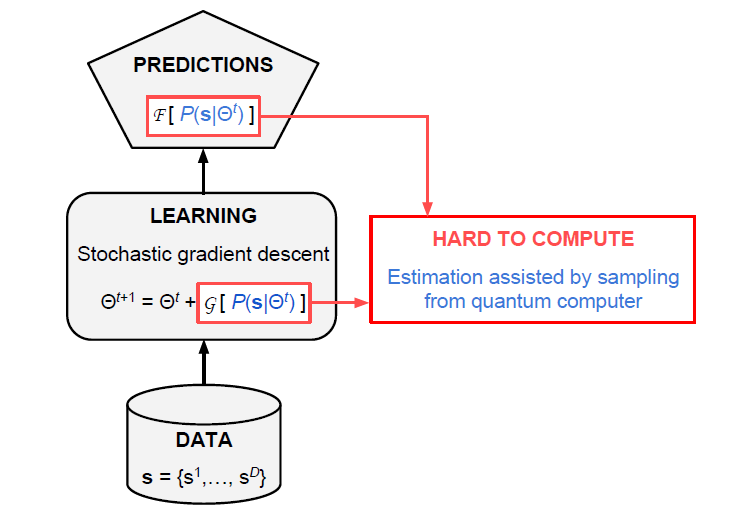
\includegraphics[width=10cm]{QML/images/3-2-1.PNG}}
\end{figure}\\


\subsubsection{Herangehensweise}

Um die begrenzten Kapazitäten von NISQ Computern ideal für Machine Learning nutzen zu können, liegt es nahe, Hybride aus Quanten- und klassischen Computern zu benutzen. Mit klassischen Computern als Steuer- bzw. Kontrolleinheit und zur Aufbereitung von Ein- und Ausgabedaten, könnte die gesamte Rechenleistung und -dauer der Quanten Computer für aufwändige ML-Algorithmen genutzt werden \cite{wittek2014quantum}.\\


Eine grundlegende Komponente in dem Hybriden Ansatz des Machine Learning ist der Informationsfluß zwischen klassischem Computer und seinem Quantum Konterpart. Jedoch stellt gerade diese essentielle Grundlage schon eine große Herausforderung dar (Eingabe- /Ausgabeproblem). Diese Schwierigkeiten wurden festgestellt bei dem Versuch, Restricted Boltzmann Maschinen (RBMs) oder auch Deep Belief Networks (DBNs) mit Quanten Geräten zu unterstützen \cite{opportunitieschallenges5}. \\

 Schafft man es jedoch, diese Hürde - neben weiteren anderen -  zu überwinden, so ist es möglich, den Lernprozess initial auf einem klassischen Computer laufen zu lassen. Dies gilt da die Model Parameter unter dem "Noise"-Level und der Präzision des Quanten Geräts liegen können. Bei Bedarf kann dann der Quanten Computer angewiesen werden, die Aufgabe zu übernehmen \cite{opportunitieschallenges5}. \\


\begin{figure}
\floatbox[{\capbeside\thisfloatsetup{capbesideposition={right},capbesidewidth=3cm}}]{figure}[\FBwidth]
{\caption{Funktionsweise eines Quantum Machine Learning Hybrids am Beispiel von Zahlenerkennung. \cite{opportunitieschallenges1}}\label{fig:test}}
{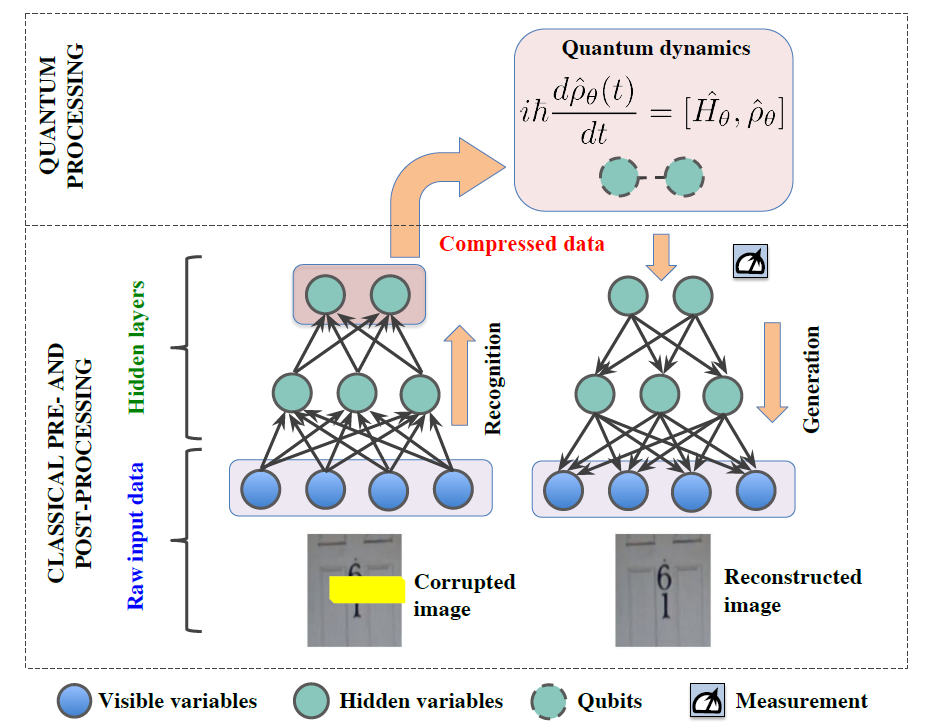
\includegraphics[width=13cm]{QML/images/3-2-2.PNG}}
\end{figure}


 Da aber mit wachsender Datenmenge die Bearbeitungsdauer von In- und Output steigt \cite{biamonte2017quantum}, wird vermutlich mit Ende der NISQ-Ära eine andere Methode hierfür gefunden werden müssen. Beim NISQ Machine Learning sind die Datenmengen aufgrund der verfügbaren Rechenkapazität der Quantencomputer allerdings sowieso sehr begrenzt, somit sollte sich diese Methode für Near-Term-Anwendungen dennoch gut eignen.\\



\include{QML/sections/Verwandte_Arbeiten}

\section{Diskussion}
\label{sec:disc}
Wir haben nun in Kapitel 3 tiefergehend die Möglichkeiten des QML im Status quo reflektiert. Vom Ziel der Quantenüberlegenheit mit Rechnern, bei denen mindestens 1000 Qubits in letztendlich Quantenregistern miteinander verschränkt werden, sind wir mit aktuellen Größen um die 65 Qubits noch sehr weit von entfernt.\\

Wir haben aber in Kapitel 2 auch gesehen, was für gewaltiges Potential das Thema QML in sich trägt. Dementsprechend lohnt es sich definitiv, weiterhin an Verbesserungen und neuen Kenntnissen zu forschen.\\
Hierbei ist großes Durchhaltevermögen gefragt. Die Quantenmechanik als Grundlage ist ein zähes Unterfangen. In Kapitel 2.1 haben wir in den theoretischen Grundlagen gesehen, wie schwer diese Art der Physik zu greifen ist. Folgerungen wie die Verschränkung oder die Heisenbergsche Unschärferelation sind sehr unintuitiv, doch ein (Haupt-)Argument der Ästhetik ist in Wissenschaften fehl am Platz.\\

Außer Acht lassen dürfen wir hierbei nicht, dass die QAML Algorithmen in der NISQ-Ära keineswegs schlecht sind. Bereits diese hybriden Algorithmen stellen, im Vergleich zu klassischen ML, eine klare Verbesserung dar.\\
Diesen Standpunkt haben wir in Kapitel 3.2 beschrieben.\\

Da diese Arbeit nur den Ansatz des Quantum Gate Models verfolgt und beschrieben hat, sei zuletzt noch angemerkt, dass es einen weiteren sehr interessanten Ansatz im Bereich des Quantum Computing gibt.\\
Es handelt sich dabei um das sogennante Quantum Annealing (QA). Der Grundgedanke hier ist heuristischer Natur zur Optimierung mithilfe von Quanten Computern - auch im Bereich des QML. Für mehr Details verweisen wir hier auf \cite{Annealing}.\\

Wir verfolgen in der Wissenschaft also bereits zwei sehr interessante Umsetzungen, um das Ziel Quantenüberlegenheit erreichen zu können. Ein logischer Schluss wäre also nun, auch nach weiteren Ansätzen zu forschen.\\
Es könnte sich durchaus ergeben, dass wir ein größeres Umsetzungs- als Hardwareproblem haben. Vielseitige Forschung ist hier deswegen sehr sinnvoll und wichtig.

%TO DO
%ca. 1 Seite
%Ausblick schreiben
\section{Schluss}
\label{sec:conclusion}
Wir befinden uns in einer spannenden Phase der Menschheitsgeschichte, Wissenschaft und Technologie sind an einem Punkt angelangt, der vor wenigen Jahrzehnten noch als undenkbar galt. Schon bald werden wir die Auswirkungen der heutigen Forschungsarbeiten auf diesem Gebiet greifen können, die Riesen der Welt der Informationstechnologie arbeiten mit Hochdruck an dem Durchbruch der Quanten Computer.\\

Auch schon in den kurzfristig kommenden Jahren erwarten uns spannende Zeiten, die NISQ-Ära verspricht uns erste große Erfolge im Bereich des QAML. Hybride Methoden bieten auf kurze Sicht eine interessante Herangehensweise an Optimierungsprobleme. Natürlich bedeuten diese noch nicht, dass die digitale und reale Welt komplett auf den Kopf gestellt wird, allerdings ist zu erwarten, dass das Arbeiten mit diesen Methoden den Weg zu großen Durchbrüchen mit Quantum Computern und Quantum Algorithmen ebnen wird.\\

Die Zukunft des Machine Learnings wird vermutlich angeführt vom Wort Quantum sein, viele Schritte sind bis zu diesem Ziel nötig, große Meilensteine sind störfreie Quantengatter, und ganz besonders Quanten Fehlerkorrektur. Trotz aller Stolpersteine und ausstehenden Erfolge schauen wir mit großer
Begeisterung den Entdeckungen und Errungenschaften der nächsten Jahre entgegen, das Potential der Quanten Technologie ist gigantisch.\\

Kleine Quantencomputer und größere für Spezialanwendungen entwickelte
Quantensimulatoren, Annealer etc. können bereits vielversprechende Anwendungen im Bereich von Machine Learning und allgemeiner Datenanalyse durchführen. Allerdings benötigen die hierfür eingesetzten Algorithmen für eine Anwendung auf große Datensätze und reale Probleme viel mehr Rechenleistung \cite{biamonte2017quantum}.\\
Kurzum benötigen sie Quanten Hardware. Hierbei stellt sich die Frage: Kann dieses Ziel erreicht werden? \\ 

Große Fortschritte sind bisher schon zu verzeichnen, es gibt Möglichkeiten für Forscher aus aller Welt um mit Quanten Computern und deren Leistung in Berührung zu kommen und somit zu ermöglichen, dass bereits jetzt eine Vielzahl kluger Köpfe an Algorithmen und Lösungen für die Zukunft arbeiten können. Ganz im Sinne von Open-Source. Dies wird in der Zukunft weiter ausgebaut werden, Quantum Cloud Computing - also der Zugriff auf Quanten Computer über die Cloud - wird verfügbar gemacht werden und der allgemeine technologische Standard von Quanten Computern wird in dieser Zeit ebenso voranschreiten, was Größe und Komplexität betrifft \cite{biamonte2017quantum}.\\

Sollten die Herausforderungen der NISQ-Ära überwunden werden, so steht einer "Quantum Zukunft" nichts mehr im Wege. Besonders die Möglichkeit der Einbindung bzw. Kombination von Quantum Machine Learning und der Kontrolle von Quantum Computern stellt einen Schritt dar, der einen sehr zügigen Fortschritt ermöglichen kann.\\ So kann der Quanten Computer bzw. das Quanten Machine Learning einer Generation verwendet werden, um die der nächsten Generation zu erschaffen, was zu einem sich selbst verstärkenden Zyklus führen kann. \\




\section*{\IfLanguageName{ngerman}{Autorenschaft}{Authorship}}
\thesisauthorship

\bibliography{references}
\bibliographystyle{plain}

\end{document}